\chapter{Heuristicas Constructivas}

\section{Heuristicas constructivas}
Para enfrentar al problema, pensamos varias heuristicas constructivas distintas. Las mismas se comentan a continuaci�n.

\subsection{Heuristica de inserci�n Greedy de nodos}
El primer enfoque que pensamos consiste en partir del dibujo original, es decir el que solo tiene los nodos cuyo orden esta
fijo e ir agregando los nuevos nodos con sus ejes, en la mejor posici�n en ese momento. Es decir, elegimos un nodo, y lo colocamos en la posici�n que genere menos cruces, teniendo en los nodos ya puestos.

Una vez hecho eso, se elige otro nodo (entre los que todavia no estan puestos) y se insertan en la misma manera.

Hay varias formas de elegir a que nodo insertar. Nosotros consideramos tres formas distintas:
\begin{enumerate}
\item Escoger un nodo al azar entre los libre
\item Escoger el nodo de mayor grado hacia el dibujo armado (es decir el nodo que tenga mas adyacentes ya colocados)
\item Escoger el nodo de menor grado hacia el dibujo armado (el nodo que tenga menos adyacentes ya colocados)
\end{enumerate}

%TODO: grafos de ejemplo
Vamos a aplicar la heuristica al siguiente grafo:

\begin{figure}[H]
    \centering
    \subfigure[]{
     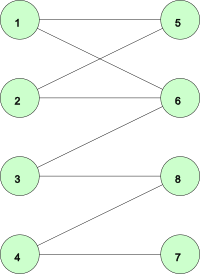
\includegraphics[scale=0.4]{./figuras/constructivas/insercionGreedyRandom/posta.png}}
     \subfigure[]{
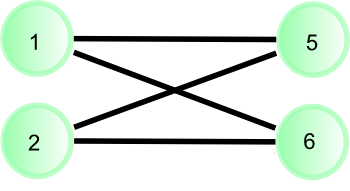
\includegraphics[scale=0.3]{./figuras/constructivas/insercionGreedyRandom/dibujo0.png} }
     \label{fig:posta}
     \caption{dibujo optimo y dibujo de partida}
\end{figure} 

\begin{itemize}

\item Insercion por selecci�n random
\begin{figure}[H]
\centering
\subfigure[]{
\includegraphics[scale=0.3]{./figuras/constructivas/insercionGreedyRandom/dibujo1.png}}
\subfigure[]{
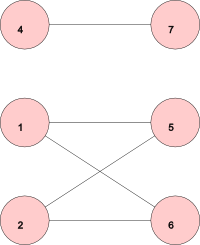
\includegraphics[scale=0.3]{./figuras/constructivas/insercionGreedyRandom/dibujo2.png} }
\subfigure[]{
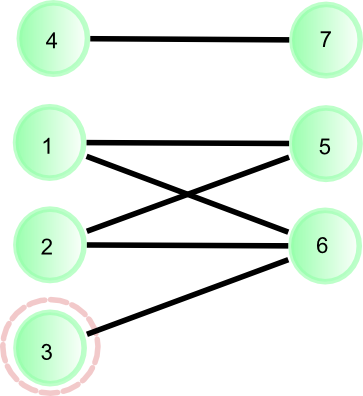
\includegraphics[scale=0.3]{./figuras/constructivas/insercionGreedyRandom/dibujo3.png}}
\subfigure[]{
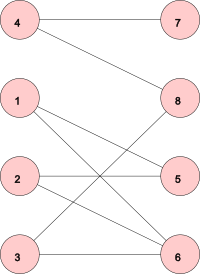
\includegraphics[scale=0.3]{./figuras/constructivas/insercionGreedyRandom/dibujo4.png}}
\end{figure}

\item Inserci�n tomando mayor grado

\begin{figure}[H]
\centering
\subfigure[]{
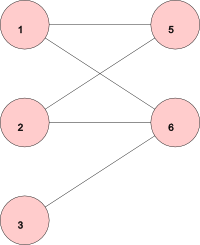
\includegraphics[scale=0.3]{./figuras/constructivas/insercionGreedyMayorGrado/dibujo1.png}}
\subfigure[]{
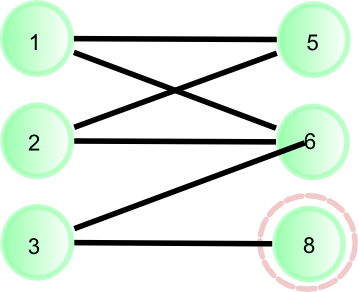
\includegraphics[scale=0.3]{./figuras/constructivas/insercionGreedyMayorGrado/dibujo2.png} }
\subfigure[]{
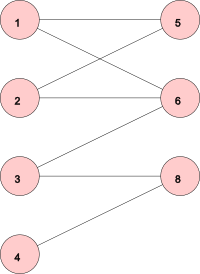
\includegraphics[scale=0.3]{./figuras/constructivas/insercionGreedyMayorGrado/dibujo3.png}}
\subfigure[]{
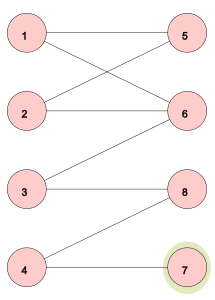
\includegraphics[scale=0.3]{./figuras/constructivas/insercionGreedyMayorGrado/dibujo4.png}}
\end{figure}

\item Insercion por menor grado
\begin{figure}[H]
\centering
\subfigure[]{
\includegraphics[scale=0.3]{./figuras/constructivas/insercionGreedyMenorGrado/dibujo1.png}}
\subfigure[]{
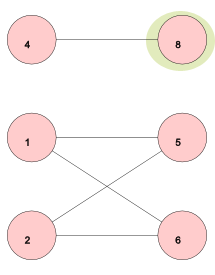
\includegraphics[scale=0.3]{./figuras/constructivas/insercionGreedyMenorGrado/dibujo2.png} }
\subfigure[]{
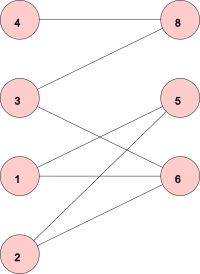
\includegraphics[scale=0.3]{./figuras/constructivas/insercionGreedyMenorGrado/dibujo3.png}}
\subfigure[]{
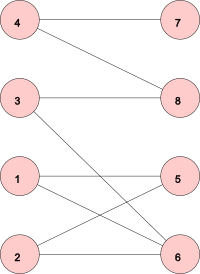
\includegraphics[scale=0.3]{./figuras/constructivas/insercionGreedyMenorGrado/dibujo4.png}}
\end{figure}
\end{itemize}

\subsubsection{Pseudocodigo}
\begin{algorithm}[H]
\caption{Propone un dibujo mediante la inserci�n golosa de nodos}
\begin{algorithmic}[1]
\PARAMS{un dibujo original, los nodos a colocar, y los ejes entre los nodos}
\WHILE{Queden nodos por poner}
\STATE nodo $\leftarrow$ elegir uno entre los nodos a poner
\STATE sacar al nodo de entre los nodos a poner
\STATE colocar al nodo en la primer posicion de su partici�n
\STATE cruces $\leftarrow$ cuantos cruces se agregan
\STATE mejorCruces $\leftarrow$ cruces
\STATE crucesPreSwap $\leftarrow$ cruces entre el nodo y el nodo siguiente en la particion
\STATE mejorPos = 0
\WHILE{No revise todas las posiciones}
\STATE mover al nodo a la proxima posici�n
\STATE crucesPreSwap $\leftarrow$ cruces entre el nodo y el nodo siguiente en la particion
\STATE cruces $\leftarrow$ cruces - crucesPreSwap + crucesPostSwap
\IF{ cruces < mejorCruces}
\STATE mejorCruces $\leftarrow$ cruces
\STATE mejorPos $\leftarrow$ la posicion donde esta ahora
\ENDIF
\STATE crucesPreSwap $\leftarrow$ crucesPostSwap
\ENDWHILE
\STATE poner al nodo finalmente en mejorPos
\ENDWHILE
\end{algorithmic}
\end{algorithm} 

Si bien no se incluye en el pseudocodigo, para no hacerlo confuso, el algoritmo mantiene un indice con la posici�n de los nodos, el cual se actualiza al hacer un ``swap'' de dos posiciones consecutivas y al fijar la posici�n final de un nodo. Esto ultimo se hace luego de insertarlo en la mejorPos y se realiza con un orden lineal en la cantidad de elementos de la partici�n cuyo indice se esta actualizando.
 
\subsubsection{Calculo de complejidad}


\subsection{Heuristica de insrcion Greedy por ejes}
Nuevamente partimos del dibujo original, pero esta vez vamos agregando ejes. Es decir tomamos un eje de los que vienen en el nuevo dibujo y lo agregamos poniendo a sus nodos en la posici�n que minimize el n�mero de cruces. Si tomamos un eje que une dos nodos que no fueron puestos aun, se agregan ambos nodos y se prueban las distintas combinaciones para minimizar los cruces. Si alguno (o ambos extremos) ya estaban puestos, se sacan ambos y se reubican. 

Esta reubicaci�n tiene mas informaci�n que la primera ubicaci�n, ya que por lo menos ambos tienen un eje ya colocado, por lo que podr'ia mejorar incluso la cantidad de cruces que habia antes de agregar el eje, cosa que con la heuristica anterior no ocurre: en la heuristica de inserci�n de nodos, cada vez que se colocaba un nodo el n�mero de cruces aumentaba o permanec�a igual; pero nunca puede bajar.

Por otro lado, si bien parecer�a que puede lograr mejores resultados que la otra heuristica, hay que tener en cuenta que va a resultar mas costosa, ya que para cada eje hay que recorrer toda la primer partici�n, y para cada posici�n de esta, se recorre la segunda, viendo cuantos cruces se originan. Por esta raz�n, es importante analizar no solo el desempe�o de esta heuristica en cuanto a reducir el n�mero de cruces, sino tambi�n en cuanto al tiempo que demora, ya que podr�a ser considerablemente mas alto que el de las dem'as heuristicas.

Si aplicamos la heuristica para fig:posta, obtenemos lo siguiente:

\begin{figure}[H]
\centering
\subfigure[]{
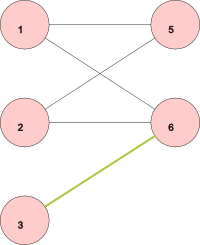
\includegraphics[scale=0.3]{./figuras/constructivas/insercionEjes/dibujo1.png}}
\subfigure[]{
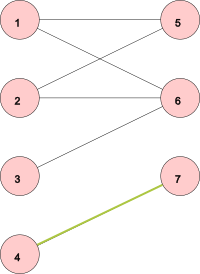
\includegraphics[scale=0.3]{./figuras/constructivas/insercionEjes/dibujo2.png} }
\subfigure[]{
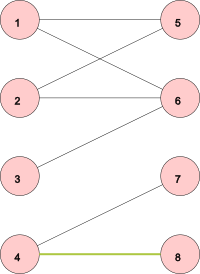
\includegraphics[scale=0.3]{./figuras/constructivas/insercionEjes/dibujo3.png}}
\subfigure[]{
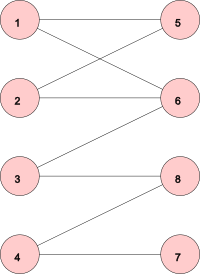
\includegraphics[scale=0.3]{./figuras/constructivas/insercionEjes/dibujo4.png}}
\end{figure}

Notemos como en el ultimo paso, agrega el eje (3,8) mueve al 8 de la posici�n que le habia asignado antes, de modo de reducir
la cantidad de cruces. Por otro lado notemos que si bien logro la soluci�n �ptima, esto se debi� a que cuando podia elegir donde poner a los nodos, los puso abajo, si hubiese elegido ponerlos arriba (opci�n valida, dado que genera la misma cantidad de cruces, es decir 0) el resultado hubiera sido distinto.

